% ds-instruc-06.tex

%-------------------------------------------------------------------------
\documentclass[11pt,a4paper]{article}
%-------------------------------------------------------------------------

%-------------------------------------------------------------------------
%-------------------------------------------------------------------------
% ds-info-S1-preambule.tex
%-------------------------------------------------------------------------

%-------------------------------------------------------------------------
\usepackage{calc}
\usepackage[text={16cm,23cm},centering=true,showframe=false]{geometry}
\usepackage{fancybox,fancyvrb,fancyhdr,lastpage,lineno,import}
\usepackage{longtable,multirow}
\usepackage{xcolor,graphics,xmpmulti,pgf,pgfpages,tikz,wrapfig}
\usepackage{colortbl,color}
\usepackage{amsmath,amssymb,amsfonts}
\usepackage{hyperref,multimedia,rotating,framed,pstricks}
\usepackage{listings,index}
%
%---- pdflatex
%\usepackage[T1]{fontenc}
%\usepackage[utf8]{inputenc}
%---- xelatex
\usepackage{fontspec}
%
%\usepackage[french]{minitoc}
\usepackage[french]{babel}
\usepackage[french]{nomencl}
\usepackage[framed,hyperref,standard]{ntheorem}
\usepackage{eurosym,pifont}
%-------------------------------------------------------------------------

%-------------------------------------------------------------------------
\lstset
{
language=Python,
basicstyle=\ttfamily,
identifierstyle=\ttfamily,
keywordstyle=\color{blue}\ttfamily,
commentstyle=\color{gray}\ttfamily,
stringstyle=\color{green}\ttfamily,
showstringspaces=false,
extendedchars=true,
numbers=left, 
numberstyle=\color{blue}\tiny,
frame=lines,
linewidth=0.95\textwidth,
xleftmargin=5mm
} 
%-------------------------------------------------------------------------

%-------------------------------------------------------------------------
\pgfdeclareimage[width=3cm,interpolate=true]{logo-enib}{logo-enib}
%-------------------------------------------------------------------------

%-------------------------------------------------------------------------
\pagestyle{fancy}
\fancyhead{}
\fancyhead[L]{\hspace*{-3em}\begin{minipage}{3cm}\pgfuseimage{logo-enib}\end{minipage}}
\fancyhead[C]{Informatique S1}
\fancyhead[R]{\thepage/\pageref{LastPage}}
\fancyfoot{}
\fancyfoot[L]{}
\fancyfoot[C]{}
\fancyfoot[R]{}
\setlength{\headheight}{80pt}
\setlength{\footskip}{38pt}
\renewcommand{\headrulewidth}{0pt}
\renewcommand{\footrulewidth}{0pt}
%-------------------------------------------------------------------------

\voffset=-1cm

%-------------------------------------------------------------------------
\def\entete{\noindent\begin{tabular}{|l|l|l|} 
\hline 
 & & \\ 
\makebox[6cm][l]{\bsc{Nom :}} & \makebox[6cm][l]{\bsc{Prénom :}} & \makebox[2.65cm][l]{\bsc{Groupe :}} \\[1mm] 
\hline 
\end{tabular}\\[1mm]
{\footnotesize \textsc{Durée : 90'\hfill Documents, calculettes, téléphones et ordinateurs interdits}}}

\def\notes{\begin{tabular}{|c|c|c|c|}  
\hline 
\makebox[0.5cm]{3} & \makebox[0.5cm]{2} & \makebox[0.5cm]{1} & \makebox[0.5cm]{0} \\  
\hline
\end{tabular}  
} 

\def\autoevaluation{$$\begin{tabular}{|c|c|c|}
\hline
\multicolumn{3}{|c|}{\textbf{Auto-évaluation}} \\
\hline
\textbf{M} & \textbf{V} & \textbf{R} \\
Méthode(s) & Vérification(s) & Résultat(s) \\
\notes & \notes & \notes \\[1mm]
\hline
\end{tabular}$$ $$ $$}

\def\reponse{\mbox{}\hfill \fbox{\huge Réponse page suivante}}
%-------------------------------------------------------------------------

%-------------------------------------------------------------------------
\tikzset{
xmin/.store in=\xmin, xmin/.default=-3, xmin=-3,
xmax/.store in=\xmax, xmax/.default=3,  xmax=3,
ymin/.store in=\ymin, ymin/.default=-3, ymin=-3,
ymax/.store in=\ymax, ymax/.default=3,  ymax=3,
}

\newcommand{\grille}{\draw[color=lightgray] (\xmin,\ymin) grid (\xmax,\ymax);}

\newcommand{\axes}{
	\draw[->] (\xmin,0) -- (\xmax,0);
	\draw[->] (0,\ymin) -- (0,\ymax);
}

\newcommand{\fenetre}{\clip (\xmin,\ymin) rectangle (\xmax,\ymax);}
%-------------------------------------------------------------------------

%-------------------------------------------------------------------------
\def\ga{\textsc{ga}}   
\def\bu{\textsc{bu}} 
\def\zo{\textsc{zo}} 
\def\meu{\textsc{meu}} 
%-------------------------------------------------------------------------

%-------------------------------------------------------------------------
\newenvironment{py}[1]{\begin{minipage}[t]{#1}\footnotesize}{\end{minipage}}
%-------------------------------------------------------------------------

%-------------------------------------------------------------------------
\input{sigle}
%-------------------------------------------------------------------------

\graphicspath{{../../fig/}}



\usepackage{epsfig}
%-------------------------------------------------------------------------

%-----------------------------------------------------------------------------
\begin{document}
%-----------------------------------------------------------------------------
\entete

%-----------------------------------------------------------------------------
\section{Exécution d'une séquence d'instructions}
%-----------------------------------------------------------------------------
Qu'affiche la séquence d'instructions suivante ?
\vspace*{5mm}

\hspace*{5mm}\begin{py}{5cm}
\begin{verbatim}
a = 729
x = 1
z = a
y = 0
t = x
print a,x,z,t,y
while x <= a: x = x*4

print a,x,z,t,y
t = x
while x > 1:
  x = x/4
  t = t/2 - x
  if t <= z: 
    z = z - t
    t = t + x*2
  y = t/2
  print a,x,z,t,y

print a,x,z,t,y
\end{verbatim}
\end{py}\hfill
\begin{tabular}[t]{|c|c|c|c|c|}
\hline
\makebox[1.25cm]{a} & \makebox[1.25cm]{x} & \makebox[1.25cm]{z} & \makebox[1.25cm]{t} & \makebox[1.25cm]{y} \\
\hline
  &   &   &   &   \\[15cm]
\hline
\end{tabular}

%-----------------------------------------------------------------------------
\newpage
\section{Calcul de $\pi$}
%-----------------------------------------------------------------------------
Ecrire un algorithme qui calcule $\pi$ à l'ordre $n$ selon la formule :
	$$\pi = 2\cdot
	\frac{4}{3}\cdot\frac{16}{15}\cdot\frac{36}{35}\cdot\frac{64}{63}\cdots =
	      2\prod_{k=1}^n\frac{4k^2}{4k^2 - 1}$$

$$\framebox[14.5cm]{\begin{minipage}{14cm}
\vspace*{17cm}

\end{minipage}}$$ 

%-----------------------------------------------------------------------------

%-----------------------------------------------------------------------------
\newpage
\section{Zéro d'une fonction}
%-----------------------------------------------------------------------------
Dans cette section, on recherche le zéro d'une fonction $f$ continue sur un 
intervalle $[a,b]$ telle que $f(a).f(b) < 0$ 
(il existe donc une racine de $f$ dans $]a,b[$ que nous supposerons 
unique). 

Ecrire un algorithme qui détermine le zéro de $\cos(x)$ dans $[1,2]$
	selon la méthode des cordes.

	Indications : on pose $x_1 = a$, $x_2 = b$ et $x = (x_2f(x_1) - x_1f(x_2))/(f(x_1)-f(x_2))$
	le point d'intersection de la corde $AB$ et de l'axe des abscisses. 
	Si $f(x_1).f(x) < 0$, la racine est dans $]x_1,x[$ et on pose $x_2 = x$; 
	sinon la racine est dans $]x,x_2[$ et on pose $x_1 = x$. 
	Puis on réitère le procédé. Lorsque $x_1$ et $x_2$ seront suffisamment 
	proches, on décidera que la racine est $x$.
$$\framebox[14.5cm]{\begin{minipage}{14cm}
\mbox{}\hfill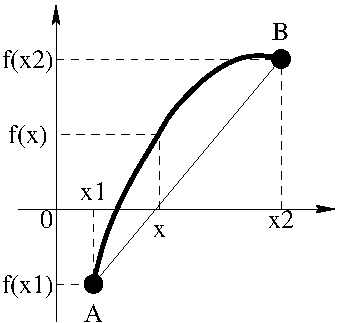
\includegraphics[width=3cm]{corde.pdf}
\vspace*{14cm}

\end{minipage}}$$ 

%-----------------------------------------------------------------------------
\newpage
\section{Le calcul Shadok}
%-----------------------------------------------------------------------------

\begin{minipage}{9.75cm}
Les cerveaux des Shadoks avaient une capacité tout à fait limitée.
Ils ne comportaient en tout que 4 cases.
Comme ils n'avaient que 4 cases, évidemment les Shadoks ne connaissaient 
pas plus de 4 mots :  {\sc ga, bu, zo et meu}.

Etant donné qu'avec 4 mots, ils ne pouvaient pas compter plus loin que 4,
le Professeur Shadoko avait réformé tout ça :
\end{minipage}
\hfill
\begin{minipage}{6cm}
\mbox{}\hfill
\includegraphics[width=4cm]{bdShadok.jpg}
\end{minipage}
\begin{itemize}
\item Quand il n'y a pas de Shadok, on dit {\sc ga} et on écrit {\sc ga}.
\item Quand il y a un Shadok de plus, on dit {\sc bu} et on écrit {\sc bu}.
\item Quand il y a encore un Shadok, on dit {\sc zo} et on écrit {\sc zo}.
\item Et quand il y en a encore un autre, on dit {\sc meu} et on écrit {\sc meu}.
\end{itemize}

Tout le monde applaudissait très fort et trouvait ça génial sauf le Devin Plombier 
qui disait qu'on n'avait pas idée d'inculquer à des enfants des bêtises pareilles 
et que Shadoko, il fallait le condamner. 
Il fut très applaudi aussi. Les mathématiques, 
cela les intéressait, bien sûr, mais brûler le professeur, c'était intéressant aussi, faut dire. 
Il fut décidé à l'unanimité qu'on le laisserait parler et qu'on le brûlerait après, à la récréation.
\begin{itemize}
\item Répétez avec moi : {\sc meu} {\sc zo} {\sc bu} {\sc ga}\ldots {\sc ga} {\sc bu} {\sc zo} {\sc meu}.
\item Et après! ricanait le Plombier.
\item Si je mets un Shadok en plus, évidemment, je n'ai plus assez 
de mots pour les compter, alors c'est très simple : on les jette dans une poubelle, 
et je dis que j'ai {\sc bu} poubelle. Et pour ne pas confondre avec le {\sc bu} du début, 
je dis qu'il n'y a pas de Shadok à côté de la poubelle et j'écris {\sc bu} {\sc ga}. 
{\sc bu} Shadok à côté de la poubelle: {\sc bu} {\sc bu}. Un autre : {\sc bu} {\sc zo}. 
Encore un autre : {\sc bu} {\sc meu}. 

On continue. {\sc zo} poubelles et pas de Shadok à côté : {\sc zo} {\sc ga}\ldots 
{\sc meu} poubelles et {\sc meu} Shadoks à côté : {\sc meu} {\sc meu}. 
Arrivé là, si je mets un Shadok en plus, il me faut une autre poubelle. 
Mais comme je n'ai plus de mots pour compter les poubelles, je m'en débarrasse 
en les jetant dans une grande poubelle. 
J'écris {\sc bu} grande poubelle avec pas de petite poubelle 
et pas de Shadok à côté: {\sc bu} {\sc ga} {\sc ga}, et on continue\ldots {\sc bu} {\sc ga} {\sc bu}, 
{\sc bu} {\sc ga} {\sc zo}\ldots {\sc meu} {\sc meu} {\sc zo}, {\sc meu} {\sc meu} {\sc meu}.
Quand on arrive là et qu'on a trop de grandes poubelles pour pouvoir les compter, 
eh bien, on les met dans une super-poubelle, on écrit {\sc bu} {\sc ga} {\sc ga} {\sc ga}, 
et on continue\ldots
\end{itemize}

\noindent\begin{enumerate}
\item Quels sont les entiers décimaux représentés en «~base Shadok~» 
	par les expressions suivantes ?
	\begin{enumerate}
	\item {\sc ga} {\sc ga}
	\item {\sc bu} {\sc bu} {\sc bu}
	\item {\sc zo} {\sc zo} {\sc zo} {\sc zo}
	\item {\sc meu} {\sc meu} {\sc meu} {\sc meu} {\sc meu} 
	\end{enumerate}	
	$$\framebox[14.5cm]{\begin{minipage}{14cm}
	\begin{tabular}{l@{ : }l}
	{\sc ga} {\sc ga} & \\[2mm]
	{\sc bu} {\sc bu} {\sc bu} & \\[2mm]
	{\sc zo} {\sc zo} {\sc zo} {\sc zo} & \\[2mm]
	{\sc meu} {\sc meu} {\sc meu} {\sc meu} {\sc meu} &
	\end{tabular}
	\end{minipage}}$$
\newpage
\item Effectuer les calculs Shadok suivants.
	\begin{enumerate}
	\item {\sc zo} {\sc zo} {\sc meu} $+$ {\sc bu} {\sc ga} {\sc meu}
	\item {\sc meu} {\sc ga} {\sc meu} $-$ {\sc bu} {\sc meu} {\sc ga}
	\item {\sc zo} {\sc meu} {\sc meu} $\times$ {\sc bu} {\sc ga} {\sc meu}
	\item {\sc zo} {\sc zo} {\sc zo} {\sc meu} $\div$ {\sc bu} {\sc ga} {\sc zo}
	\end{enumerate}
	$$\framebox[14.5cm]{\begin{minipage}{14cm}
	\begin{tabular}{l@{ : }l}
	{\sc zo} {\sc zo} {\sc meu} $+$ {\sc bu} {\sc ga} {\sc meu} & \\[2mm]
	{\sc meu} {\sc ga} {\sc meu} $-$ {\sc bu} {\sc meu} {\sc ga} & \\[2mm]
	{\sc zo} {\sc meu} {\sc meu} $\times$ {\sc bu} {\sc ga} {\sc meu} & \\[2mm]
	{\sc zo} {\sc zo} {\sc zo} {\sc meu} $\div$ {\sc bu} {\sc ga} {\sc zo}
	\end{tabular}
	\end{minipage}}$$
\end{enumerate}

%-----------------------------------------------------------------------------
\label{fini}
\end{document}
%-----------------------------------------------------------------------------
